% Resumen del trabajo de grado (6-7 páginas). Compila con pdflatex, sin biber.
% En Overleaf: Menu > Main document > resumen_ejecutivo.tex para compilarlo.
\documentclass[11pt,letterpaper]{article}
\usepackage[utf8]{inputenc}
\usepackage[T1]{fontenc}
\usepackage[spanish,es-tabla,es-nodecimaldot]{babel}
\usepackage[margin=2.3cm]{geometry}
\usepackage{lmodern}
\usepackage{graphicx}
\usepackage{booktabs}
\usepackage{array}
\usepackage{tabularx}
\usepackage{enumitem}
\usepackage{float}
\usepackage{caption}
\usepackage{xcolor}
\usepackage{titlesec}
\usepackage{amsmath,amssymb}
\usepackage[hidelinks]{hyperref}
\graphicspath{{Figuras/}}

\definecolor{gris}{HTML}{434E5A}
\definecolor{turquesa}{HTML}{2FA89C}
\titleformat{\section}{\large\bfseries\color{gris}}{\thesection.}{0.5em}{}
\titleformat{\subsection}{\normalsize\bfseries\color{gris}}{\thesubsection}{0.5em}{}
\titlespacing*{\section}{0pt}{9pt}{4pt}
\titlespacing*{\subsection}{0pt}{6pt}{2pt}
\captionsetup{font=small,labelfont=bf}
\setlength{\parskip}{0.45em}
\setlength{\parindent}{0pt}
\setlist{itemsep=1pt,topsep=2pt}
\newcolumntype{Y}{>{\raggedright\arraybackslash}X}
\newcommand{\cmark}{\ensuremath{\checkmark}}

\begin{document}

\begin{center}
{\Large\bfseries\color{gris} Integración de una herramienta basada en modelos de lenguaje de gran tamaño a una arquitectura UNS para analítica de datos en Industria~4.0}\\[6pt]
{\large Resumen del trabajo de grado}\\[8pt]
Norbey Camilo Infante Villamil\\
Maestría en Ingeniería de Telecomunicaciones, Universidad Industrial de Santander\\
Director: Ph.D. Juan Manuel Rey \quad Codirector: Ph.D. Homero Ortega Boada\\
Empresa aliada: DAUTOM S.A.S.\\[2pt]
{\color{turquesa}\rule{0.35\textwidth}{2pt}}
\end{center}

\section{Problema y propósito}

Las plantas que avanzan hacia la Industria~4.0 producen grandes volúmenes de datos desde fuentes heterogéneas (PLC, SCADA, MES, ERP), con frecuencia fragmentados y sin un significado explícito \cite{wef1,scd1}. La arquitectura \textit{Unified Namespace} (UNS) centraliza y estructura esa información en tiempo real sobre la jerarquía de ISA-95 \cite{DiazUNS2025,johnsson2004isa}, pero centralizar no basta para aprovecharla: consultarla sigue exigiendo conocer la estructura de los datos y las herramientas para extraerlos.

Péter y Werner \cite{Thesis2024UNS} estudiaron el UNS como repositorio centralizado con contexto semántico y señalaron la inteligencia artificial sobre datos contextualizados como trabajo futuro, sin implementarla ni medirla. Este trabajo aborda ese vacío: integra un modelo de lenguaje de gran tamaño (LLM) a una arquitectura UNS para que un usuario de planta consulte en lenguaje natural el estado actual y el histórico de la producción, y mide el desempeño del sistema resultante.

\textbf{Objetivo general.} Integrar una herramienta basada en LLM para la analítica de datos de una arquitectura UNS aplicada a un caso de Industria~4.0. Los objetivos específicos fueron: caracterizar el caso de estudio y sus requerimientos (OE1); diseñar e implementar el UNS (OE2); seleccionar el mecanismo de integración y la herramienta LLM (OE3); integrar la herramienta al UNS con el contexto del caso (OE4); y validar el sistema con métricas de desempeño (OE5).

\textbf{Metodología.} Estudio de caso único de tipo instrumental, en dos fases: una descriptivo-comparativa, que contrastó los mecanismos de integración disponibles, y una experimental, que implementó el mecanismo seleccionado y lo validó con métricas definidas a priori (precisión y F1, latencia, calidad semántica y tasa de alucinaciones).

\section{Caso de estudio y requerimientos (OE1)}

El caso se inspira en un proyecto de integración IIoT que DAUTOM S.A.S. realizó en una empresa molinera de Barranquilla, y que conectó las áreas de empaque de harina de maíz y de trigo a un MES sobre Ignition. Cada área tiene dos líneas (A y B), y cada línea dos empacadoras y una enfardadora. Las empacadoras tienen PLC Omron que entregan conteo, tiempo de ciclo y estado por Modbus TCP; las enfardadoras aportan señales de entrada y salida. Un PLC Weidmüller por área concentra los datos y los envía por OPC UA al Gateway de Ignition, donde el MES gestiona órdenes de trabajo (WO) y corridas y calcula disponibilidad, rendimiento, calidad y OEE.

Del análisis del caso surgieron tres requerimientos y ocho desafíos de analítica (Tabla~\ref{tab:req}), que guiaron el diseño y sirvieron después como criterio de validación.

\begin{table}[H]
\centering\small
\caption{Requerimientos y desafíos de analítica identificados en el caso de estudio.}\label{tab:req}
\begin{tabularx}{\textwidth}{@{}p{4.2cm}Y@{}}
\toprule
\textbf{Requerimiento} & \textbf{Desafíos} \\
\midrule
R1. Interpretar consultas en lenguaje natural con conocimiento del dominio &
D1.1 términos técnicos ambiguos (disponibilidad, rendimiento); D1.2 relaciones causales entre variables; D1.3 mapeo del lenguaje natural a la jerarquía del namespace. \\
R2. Generar reportes con análisis comparativos &
D2.1 elegir comparaciones relevantes; D2.2 combinar UNS, MES e histórico; D2.3 adaptar el reporte al perfil del usuario. \\
R3. Acceder de forma eficiente a datos históricos y en tiempo real &
D3.1 consultas eficientes a la base de datos; D3.2 granularidad temporal según el rango consultado. \\
\bottomrule
\end{tabularx}
\end{table}

\section{Arquitectura UNS (OE2)}

La literatura describe dos métodos para estructurar un UNS: el de Schultz, con varios brokers MQTT por nivel, y el de Parris, con un único broker y la jerarquía codificada en el tópico \cite{DiazUNS2025}. El caso usa OPC UA y no MQTT, pero el principio que separa ambos métodos es independiente del protocolo. Como toda la planta reporta a un único servidor Ignition, se adoptó el principio de Parris: un único Tag Provider, \texttt{UNS\_Molinera}, con la jerarquía Enterprise--Site--Area--Line--Cell de ISA-95 (Molinera / Barranquilla / Empaque Maíz y Empaque Trigo / Línea A y B / Empacadora 1, Empacadora 2 y Enfardadora).

Dentro de cada línea, los datos se organizan por dominio funcional mediante cuatro plantillas UDT: \texttt{ERP} (nivel 4: orden activa, cantidades y tiempos programados), \texttt{MES} (nivel 3: OEE y su desglose, conteos, tasas y tiempos de la corrida), \texttt{Line} (niveles 1--2: estado, tiempo de ciclo y los contadores acumulados Infeed, Outfeed y Waste, en fardos) y \texttt{Edge} (nivel 0, por celda: Infeed, Outfeed, Waste y Status). De \texttt{Edge} se derivaron los UDT \texttt{Empacadora} y \texttt{Enfardadora}, con la misma estructura, para que cada equipo declare la unidad de sus conteos: bolsas en la Empacadora y fardos en la Enfardadora. Cada plantilla se define una vez y se instancia en las cuatro líneas y las doce celdas. Los valores de prueba se generaron con scripts, de modo que la validación de esta fase se centró en la fidelidad de la estructura al diseño.

\section{Selección del mecanismo y de la herramienta LLM (OE3)}

Se compararon tres mecanismos de integración de un LLM con sistemas externos: invocación directa por HTTP/REST, pipelines de orquestación y \textit{Model Context Protocol} (MCP) \cite{MastouriRESTtoMCP2026,EhteshamAgentProtocols2025,anthropic2024intro}, frente a seis criterios derivados de la propuesta, de los requerimientos y de buenas prácticas (Tabla~\ref{tab:mec}).

\begin{table}[H]
\centering\small
\caption{Comparación de mecanismos de integración (\cmark\cmark{} robusto, \cmark{} parcial, $\times$ limitación significativa).}\label{tab:mec}
\begin{tabular}{@{}lccc@{}}
\toprule
\textbf{Criterio} & \textbf{HTTP/REST} & \textbf{Pipelines} & \textbf{MCP} \\
\midrule
Acceso en tiempo real & \cmark & $\times$ & \cmark\cmark \\
Acción bidireccional & \cmark & $\times$ & \cmark\cmark \\
Privacidad IIoT & \cmark\cmark & \cmark & $\times$ \\
Contexto semántico & $\times$ & \cmark & \cmark\cmark \\
Esfuerzo de desarrollo y mantenimiento & $\times$ & $\times$ & \cmark\cmark \\
Interoperabilidad multi-proveedor & \cmark & $\times$ & \cmark\cmark \\
\bottomrule
\end{tabular}
\end{table}

MCP resultó favorable en cinco de los seis criterios: el modelo descubre en tiempo de ejecución qué herramientas y datos existen, y cada dato puede viajar con su significado mediante las primitivas \textit{Tools} y \textit{Resources} \cite{anthropic2024arch}. Su desventaja es la privacidad, con una superficie de amenazas documentada \cite{HouMCPLandscape2025}. Se aceptó como riesgo y se mitigó con tres decisiones de diseño: transporte local STDIO, alcance de solo lectura limitado a los contextos del UNS y autenticación OAuth si en el futuro se requiere transporte remoto. Como herramienta LLM se seleccionó Claude (Anthropic) por tres criterios de adaptabilidad: soporte nativo de MCP como anfitrión, capacidad de encadenar varias invocaciones de herramientas en una respuesta (patrón ReAct \cite{YaoReAct2023}) y aptitud para traducir el vocabulario de planta en español a los nombres de tags del UNS.

\section{Integración del LLM al UNS (OE4)}

La Figura~\ref{fig:arq} resume la arquitectura implementada. Tiene cuatro piezas.

\begin{figure}[H]
\centering
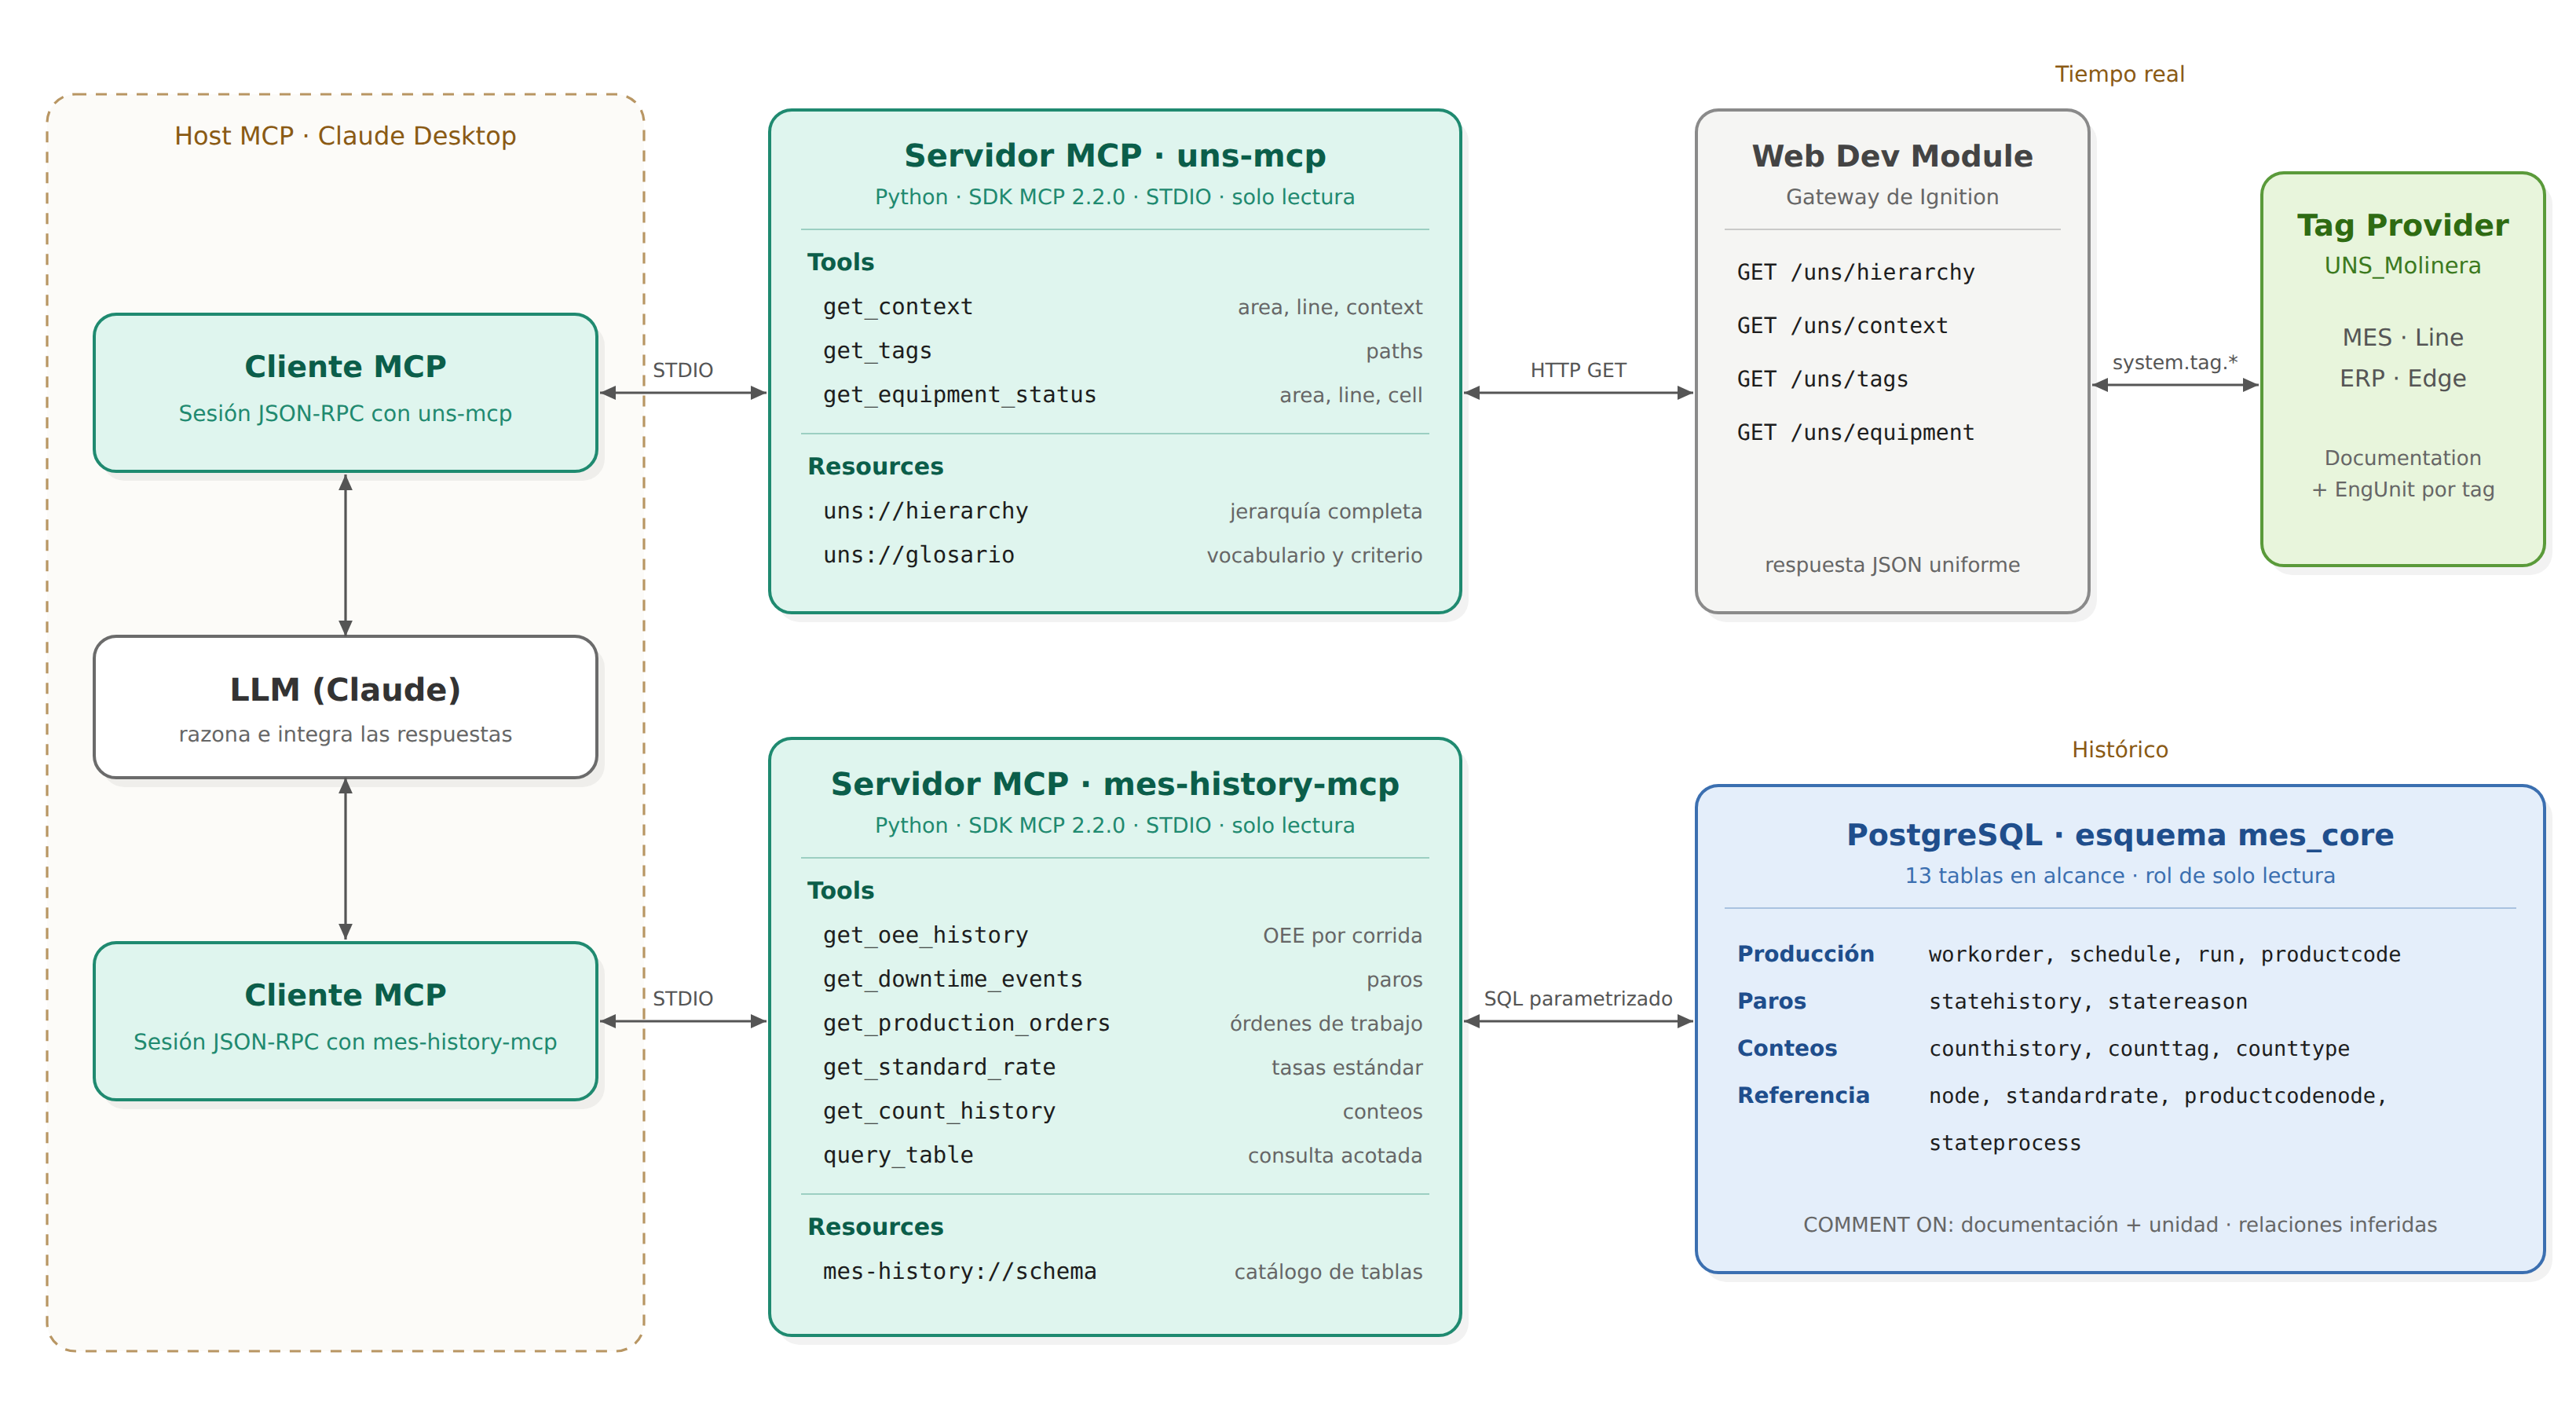
\includegraphics[width=0.92\textwidth]{arquitectura_mcp_implementada.png}
\caption{Arquitectura implementada: Claude Desktop como anfitrión MCP, dos servidores MCP independientes y sus fuentes de datos.}\label{fig:arq}
\end{figure}

\textbf{Capa de endpoints y modelado semántico.} Para no exponer el Gateway completo, se construyó sobre el Web Dev Module de Ignition \cite{ignition_webdev} una capa de cuatro endpoints HTTP de solo lectura (\texttt{/uns/hierarchy}, \texttt{/uns/context}, \texttt{/uns/tags} y \texttt{/uns/equipment}) con validación de parámetros y códigos de error explícitos. El significado de cada tag se cargó en la propia fuente, en los campos \texttt{Documentation} y \texttt{EngUnit} de las plantillas UDT, siguiendo el principio de anotar la semántica en el modelo de datos industrial \cite{KattiOPCUASemantics2018}. Cada unidad se validó contra los valores reales del Tag Provider.

\textbf{Servidor \texttt{uns-mcp} (tiempo real).} Implementado en Python con el SDK oficial de MCP y transporte STDIO, expone tres Tools (\texttt{get\_context}, \texttt{get\_tags} y \texttt{get\_equipment\_status}) y el Resource \texttt{uns://hierarchy}. Cada valor llega al modelo con su ruta, su documentación, su unidad, su calidad y su marca de tiempo.

\textbf{Servidor \texttt{mes-history-mcp} (histórico).} Atiende el requerimiento R3 conectándose al esquema \texttt{mes\_core} de PostgreSQL con un rol de solo lectura sobre trece tablas. La semántica se cargó con \texttt{COMMENT ON}. Expone seis Tools (OEE, paros, órdenes, tasas estándar, conteos y una consulta acotada, \texttt{query\_table}, que nunca recibe SQL libre) y el Resource \texttt{mes-history://schema}. La granularidad se decide en el servidor y no en el modelo: hasta 2~h por minuto, hasta 48~h por hora y por encima de ese límite por día, con agregación en SQL que recalcula las razones del OEE en lugar de promediarlas y un límite de 1000 filas por respuesta.

\textbf{Contextualización del modelo.} En lugar de instrucciones en el cliente o de un \textit{Prompt} MCP, se usaron Resources que viajan con cada servidor: \texttt{uns://glosario}, generado en cada lectura desde el Tag Provider, con el vocabulario de la planta y el criterio para elegir servidor, y \texttt{mes-history://schema}, con el mapa del esquema relacional. Así, ante una pregunta que combina el estado actual y el histórico, el LLM la divide entre los dos servidores, convierte el OEE a una misma escala gracias a la unidad que acompaña cada dato (porcentaje en el UNS, fracción en el histórico) y redacta una sola respuesta, sin que los servidores se comuniquen entre sí.

\section{Validación del sistema integrado (OE5)}

\textbf{Diseño.} La validación comprueba que la integración funciona; no compara ni evalúa el modelo. Se construyó un banco de 25 preguntas en seis categorías (tiempo real, histórica, combinada, ambigua, causal y sin datos), cada una asociada al desafío que pone a prueba y con una respuesta de referencia calculada fuera del sistema: con SQL directo sobre \texttt{mes\_core} para el histórico, y con lecturas de los tags antes y después de cada ejecución para el tiempo real. Cada pregunta se ejecutó tres veces en conversaciones nuevas en modo incógnito, para 75 ejecuciones, con Claude Desktop, el modelo Opus~5.5 y una única configuración. La precisión mide la proporción de respuestas con todos sus datos clave correctos; el F1 se calcula sobre los datos clave individuales; una alucinación es una cifra, un nombre, un estado o una causa inventados, es decir, ausentes de las salidas de las Tools y de los datos \cite{Ji2023Hallucination}, mientras que un error al resumir o comparar datos que sí existen se registra en la coherencia; la latencia se midió de extremo a extremo con un script que automatiza el cliente; y la calidad semántica se puntuó de 1 a 5 en coherencia, pertinencia y suficiencia con una rúbrica definida de antemano, que aplicó el tutor técnico de DAUTOM.

\begin{table}[H]
\centering\small
\caption{Resultados por categoría (75 ejecuciones). Latencia en segundos; calidad en escala 1--5.}\label{tab:res}
\begin{tabular}{@{}lcccccc@{}}
\toprule
\textbf{Categoría} & \textbf{Ejec.} & \textbf{Precisión} & \textbf{F1} & \textbf{Alucin.} & \textbf{Latencia media / P95} & \textbf{Calidad} \\
\midrule
Tiempo real & 12 & 100,0\,\% & 1,000 & 0 & 16,1 / 23,5 & 4,58 \\
Histórica & 24 & 91,7\,\% & 0,922 & 0 & 16,0 / 30,1 & 4,76 \\
Combinada & 12 & 91,7\,\% & 0,958 & 0 & 18,2 / 25,4 & 4,67 \\
Ambigua & 9 & 88,9\,\% & --- & 0 & 28,1 / 58,6 & 4,70 \\
Causal & 9 & 100,0\,\% & 0,988 & 0 & 43,0 / 68,6 & 4,67 \\
Sin datos & 9 & 100,0\,\% & --- & 0 & 19,7 / 31,7 & 4,67 \\
\midrule
\textbf{Total} & \textbf{75} & \textbf{94,7\,\%} & \textbf{0,958} & \textbf{0} & \textbf{21,5 / 50,9} & \textbf{4,69} \\
\bottomrule
\end{tabular}
\end{table}

\textbf{Resultados.} El sistema respondió correctamente 71 de 75 ejecuciones (94,7\,\%), con F1 de 0,958 sobre los datos clave y ninguna alucinación: las cifras adicionales que agregó el modelo se verificaron contra los datos y coinciden, y en las preguntas sin datos reconoció que no había registros. La latencia media fue de 21,5~s (mediana 17,1~s), de los cuales los servidores MCP ocuparon 2,2~s en promedio; el resto lo consumió el modelo al razonar y redactar. Las preguntas causales y ambiguas fueron las más lentas porque requirieron más llamadas a las Tools (5,9 y 4,3 por ejecución). La calidad semántica promedió 4,69; la pertinencia fue el criterio más bajo (4,28) porque el cliente tiende a agregar análisis no solicitado, como desgloses diarios o hipótesis de causa.

Tres de las cuatro respuestas incorrectas se debieron a un defecto de la Tool \texttt{get\_production\_orders}: al recibir la fecha final sin hora la interpretaba como las 00:00 y omitía las órdenes iniciadas ese día (18 órdenes en lugar de 21). El defecto se corrigió después de la validación, junto con la documentación de las unidades de conteo, y ambas correcciones se comprobaron con un banco adicional de 10 preguntas y 30 ejecuciones: las 30 fueron correctas, sin alucinaciones y con una latencia media de 13,8~s. La cuarta respondió la producción de las corridas iniciadas en el día y no la del día calendario, dos definiciones válidas de «producción del día». Ningún error se originó en una cifra inventada por el modelo.

\textbf{Cumplimiento de los desafíos.} Cuatro desafíos se cumplieron sin fallos (D1.1, D1.2, D2.1 y D3.2), dos con una salvedad atribuible a la Tool de órdenes o al criterio de conteo (D1.3, 15 de 18; D2.2, 11 de 12), D3.1 se cumple por diseño (consultas parametrizadas, agregación en SQL, límite de filas y rol de solo lectura) y D2.3, la adaptación del reporte al perfil del usuario, no se implementó. En consecuencia, la integración cumple los requerimientos del caso de estudio, salvo la adaptación del reporte al perfil del usuario (D2.3), que queda como trabajo futuro.

\section{Conclusiones}

El trabajo se propuso integrar una herramienta basada en un LLM a una arquitectura UNS para la analítica de datos de un caso de Industria~4.0, y esa integración se logró. En el entorno de prueba, un usuario pregunta en español y con el vocabulario de la planta por el estado actual de una línea, por su historial o por ambos, y recibe una respuesta respaldada por los datos del UNS y de la base \texttt{mes\_core}.

\begin{itemize}
\item \textbf{Aporte.} Un mecanismo concreto para que un LLM consulte un UNS sin sustituirlo como fuente de verdad. El significado de los datos, que en un UNS ya está en la jerarquía, los nombres y las unidades, llega al modelo a través de MCP y no hay que reconstruirlo en cada pregunta. Las Tools acotadas y de solo lectura limitan el acceso del modelo a un conjunto pequeño de operaciones cuyo alcance se conoce de antemano, lo que permite revisar el riesgo de la integración.
\item \textbf{Dónde queda el riesgo.} Los errores observados no se originaron en una cifra inventada por el modelo, sino en una Tool y en una expresión con dos definiciones. El modelo confía en lo que devuelve la Tool y lo presenta con seguridad, de modo que la confiabilidad de las respuestas depende de la calidad de las Tools y de sus metadatos, y su verificación con referencias independientes debe ser parte del diseño.
\item \textbf{Costo de ampliar.} Corregir un defecto o atender un tipo de pregunta nuevo consiste en ajustar o agregar una Tool, sin cambiar la arquitectura ni el modelo, como mostró la corrección validada en el banco adicional.
\end{itemize}

\textbf{Alcance y límites.} Los valores de los tags y los registros históricos se generaron con scripts que respetan la estructura, las unidades y las reglas de negocio del caso real, pero no provienen de una planta en operación; por eso no se probó el comportamiento ante el ruido y los vacíos de datos reales, y el simulador no reproduce todas las relaciones entre variables, como la de la tasa estándar con la producción. La validación usó un único modelo y una única configuración, porque su objetivo era comprobar la integración: los porcentajes describen este sistema sobre este banco y no se extienden a otros modelos ni a otras plantas. La latencia depende del cliente y de la red del equipo de pruebas.

\textbf{Trabajo futuro.} Fijar la definición de producción diaria y repetir el banco completo para confirmar todas las correcciones; validar con datos de una planta en operación y, mientras tanto, ajustar el simulador para que conserve las relaciones entre variables; implementar la adaptación de las respuestas al perfil del usuario (D2.3); extender la misma estructura de Tools y Resources a otras fuentes, como mantenimiento o calidad; y, si el caso lo justifica, estudiar la escritura controlada sobre el UNS con confirmación humana y permisos propios.

{\small
\begin{thebibliography}{99}\setlength{\itemsep}{1pt}
\bibitem{wef1} World Economic Forum, ``Unlocking the full potential of digital transformation through technology and talent,'' 2024. [Online]. Available: \url{https://www.weforum.org/stories/2024/09/unlocking-the-full-potential-of-digital-transformation-through-technology-and-talent}
\bibitem{scd1} P. Li, Y. Chen, and X. Guo, ``Digital transformation and supply chain resilience,'' \textit{Int. Rev. Econ. Finance}, vol. 99, Art. no. 104033, 2025, doi: 10.1016/j.iref.2025.104033.
\bibitem{DiazUNS2025} J. A. Díaz, J. M. Rey, I. Hernández, N. Duarte, and W. Reynolds, ``Unified Namespace: A new paradigm for industrial IoT data integration,'' \textit{IEEE Internet Things Mag.}, 2025, doi: 10.1109/MIOT.2025.3633944.
\bibitem{johnsson2004isa} C. Johnsson, ``ISA 95 -- how and where can it be applied,'' \textit{ISA Expo}, pp. 1--10, 2004.
\bibitem{Thesis2024UNS} Á. Péter and S. Werner, ``The impact of Unified Namespace in Industry 4.0,'' M.S. thesis, Dept. Automatic Control, Lund Univ., Lund, Sweden, 2024.
\bibitem{MastouriRESTtoMCP2026} M. Mastouri, E. Ksontini, A. Barrak, and W. Kessentini, ``From REST to MCP: An empirical study of API wrapping and automated server generation for LLM agents,'' \textit{ACM Trans. Softw. Eng. Methodol.}, 2026, arXiv:2507.16044.
\bibitem{EhteshamAgentProtocols2025} A. Ehtesham, A. Singh, G. K. Gupta, and S. Kumar, ``A survey of agent interoperability protocols: MCP, ACP, A2A, and ANP,'' 2025, arXiv:2505.02279.
\bibitem{anthropic2024intro} Anthropic, ``What is the Model Context Protocol (MCP)?,'' 2024. [Online]. Available: \url{https://modelcontextprotocol.io/docs/getting-started/intro}
\bibitem{anthropic2024arch} Anthropic, ``Architecture overview -- Model Context Protocol,'' 2024. [Online]. Available: \url{https://modelcontextprotocol.io/docs/learn/architecture}
\bibitem{HouMCPLandscape2025} X. Hou, Y. Zhao, S. Wang, and H. Wang, ``Model Context Protocol (MCP): Landscape, security threats, and future research directions,'' 2025, arXiv:2503.23278.
\bibitem{YaoReAct2023} S. Yao \textit{et al.}, ``ReAct: Synergizing reasoning and acting in language models,'' in \textit{Proc. ICLR}, 2023.
\bibitem{ignition_webdev} Inductive Automation, ``Web Dev -- Ignition user manual,'' 2025. [Online]. Available: \url{https://docs.inductiveautomation.com/docs/8.3/ignition-modules/web-dev}
\bibitem{KattiOPCUASemantics2018} A.-K. Katti and C. Plociennik, ``SA-OPC-UA: Introducing semantics to OPC-UA application methods,'' in \textit{Proc. IEEE CASE}, 2018, doi: 10.1109/COASE.2018.8560467.
\bibitem{Ji2023Hallucination} Z. Ji \textit{et al.}, ``Survey of hallucination in natural language generation,'' \textit{ACM Comput. Surv.}, vol. 55, no. 12, pp. 1--38, 2023, doi: 10.1145/3571730.
\end{thebibliography}
}

\end{document}
